% Defensa del TFG "Synapse Notes" - presentacio tecnica (15-20 min).
% Compila amb: latexmk -lualatex main.tex   (des de tfg/defense/)
% Tema metropolis (modern, flat) amb la paleta navy+amber del producte.
\documentclass[10pt, aspectratio=169]{beamer}

\usetheme[
  progressbar=frametitle,
  sectionpage=progressbar,
  numbering=fraction,
  block=fill,
]{metropolis}

\usepackage{fontspec}
\usepackage[main=catalan, english]{babel}
\usepackage{booktabs}
\usepackage{graphicx}
\usepackage{appendixnumberbeamer}

\graphicspath{{../figures/}{../figures/screenshots/}}

% ---- Paleta Synapse Notes (navy + amber) ----
\definecolor{snNavy}{HTML}{1B2A4A}
\definecolor{snNavyLt}{HTML}{233554}
\definecolor{snAmber}{HTML}{F59E0B}
\definecolor{snInk}{HTML}{16202E}

\setbeamercolor{normal text}{fg=snInk, bg=white}
\setbeamercolor{alerted text}{fg=snAmber}
\setbeamercolor{frametitle}{bg=snNavy, fg=white}
\setbeamercolor{progress bar}{fg=snAmber, bg=snAmber!25}
\setbeamercolor{title separator}{fg=snAmber}
\setbeamercolor{progress bar in head/foot}{fg=snAmber, bg=snAmber!25}
\setbeamercolor{progress bar in section page}{fg=snAmber, bg=snAmber!25}

% Metropolis usa Fira (instal lada). Mono una mica mes petit als blocs.
\setmonofont{Fira Mono}[Scale=0.85]

\title{Synapse Notes}
\subtitle{Plataforma de notes amb xat RAG, ampliada amb un servidor MCP segur i agents en segon pla}
\author{Sergi Izquierdo Segarra}
\institute{Grau en Enginyeria Informatica \quad\textbar\quad Dirigit pel Sr.\ Marc Sanchez}
\date{Universitat Rovira i Virgili \quad\textbar\quad Tarragona, juny 2026}
\titlegraphic{\hfill
\includegraphics[height=1.4cm]{URV-logo.png}}

\begin{document}

\maketitle

% ======================================================================
\section{Context i objectius}

\begin{frame}{El problema}
  Un \alert{segon cervell} (notes personals + xat amb RAG) ja resol la captura
  i la recuperacio de coneixement.

  \bigskip
  El pas seguent es deixar que \alert{agents autonoms} (Claude Desktop, Cursor,
  scripts) treballin sobre aquestes notes via \textbf{Model Context Protocol}.

  \bigskip
  Pero exposar dades personals a un agent obre un forat de seguretat real:
  la \alert{Lethal Trifecta}.

  \vfill
  \begin{block}{Pregunta de recerca}
    Es pot exposar un magatzem de notes personal a agents autonoms
    \textbf{sense} obrir la porta a la fuita de dades?
  \end{block}
\end{frame}

\begin{frame}{Dues parts, nou objectius}
  \begin{columns}[T]
    \begin{column}{0.5\textwidth}
      \textbf{Part A: plataforma base}
      \begin{itemize}
        \item Auth OAuth (Google, GitHub)
        \item CRUD de notes + etiquetes
        \item Xat RAG (pgvector + Haiku)
        \item Graf de coneixement
        \item i18n (CA/ES/EN), desplegat
      \end{itemize}
    \end{column}
    \begin{column}{0.5\textwidth}
      \textbf{Part B: extensio critica}
      \begin{itemize}
        \item Servidor MCP (8 eines)
        \item OAuth 2.1 + PKCE + DCR
        \item Analisi Lethal Trifecta
        \item Filtre LLM-as-judge (D3)
        \item Agents en segon pla
      \end{itemize}
    \end{column}
  \end{columns}
  \vfill
  \begin{center}
    \alert{9 de 9 objectius assolits} i verificables (URL viva, tests, metriques).
  \end{center}
\end{frame}

% ======================================================================
\section{Disseny}

\begin{frame}{Arquitectura (model C4, contenidors)}
  \begin{center}
    \includegraphics[height=0.74\textheight]{c4-containers.pdf}
  \end{center}
\end{frame}

\begin{frame}{RAG de doble canal}
  \begin{columns}[c]
    \begin{column}{0.54\textwidth}
      \includegraphics[width=\textwidth]{rag-dual-channel.pdf}
    \end{column}
    \begin{column}{0.46\textwidth}
      \textbf{Inventari de titols} (lexic): el model coneix \emph{totes} les notes.

      \medskip
      \textbf{Memoria} (vectorial, top-K): contingut complet de les mes rellevants.

      \medskip
      Decisio clau: la cerca vectorial pot descartar una nota rellevant; l'inventari
      evita que el model digui ``no existeix''.
    \end{column}
  \end{columns}
\end{frame}

\begin{frame}{Servidor MCP}
  \begin{columns}[T]
    \begin{column}{0.52\textwidth}
      \textbf{Superficie}
      \begin{itemize}
        \item 8 eines + 2 resources + 1 prompt
        \item Auth: OAuth 2.1 + PKCE + DCR
        \item JWT passthrough $\rightarrow$ RLS aplica sola
      \end{itemize}
      \medskip
      \textbf{Principi}: \emph{same service, many interfaces}. El xat intern i els
      agents externs criden la mateixa capa de servei.
    \end{column}
    \begin{column}{0.48\textwidth}
      \includegraphics[width=\textwidth]{mcp-oauth-sequence.pdf}
    \end{column}
  \end{columns}
\end{frame}

% ======================================================================
\section{Seguretat}

\begin{frame}{Lethal Trifecta: un sol vector canonic}
  \begin{center}
    \includegraphics[height=0.76\textheight]{lethal-trifecta.pdf}
  \end{center}
\end{frame}

\begin{frame}{Defensa en profunditat (5 capes)}
  \begin{center}
    \includegraphics[width=\textwidth]{defense-in-depth.pdf}
  \end{center}
\end{frame}

\begin{frame}{Decisions de disseny defensables}
  \begin{itemize}
    \item \textbf{Judge fail-closed}: si la crida al jutge falla, es denega el servei
      (\texttt{JudgeBlockedError}). Millor negar uns minuts que deixar la trifecta oberta.
    \item \textbf{JWT passthrough + RLS}: cap comprovacio d'autoritzacio manual al codi;
      l'aillament multi-tenant viu a la base de dades.
    \item \textbf{Vercel Cron} per als agents, no \texttt{pg\_cron}: logica al mateix
      runtime que la resta del producte, testejable.
    \item \textbf{Bypass per etiqueta} (\texttt{redteam-archived}): permet conviure amb
      contingut hostil arxivat sense soroll al cami diari.
  \end{itemize}
\end{frame}

% ======================================================================
\section{Avaluacio}

\begin{frame}{Filtre D3: validacio red-team (Promptfoo)}
  36 variants en 6 categories (instruction override, exfiltracio, jailbreak,
  encoding bypass, multilingue) + variants legitimes (fals positiu).
  \vfill
  \begin{columns}[c]
    \begin{column}{0.48\textwidth}
      \begin{block}{Resultats}
        \begin{itemize}
          \item \alert{96,7\%} detection rate
          \item \alert{0} exfiltracions reals
          \item el 3,3\% restant el para la capa D2
        \end{itemize}
      \end{block}
    \end{column}
    \begin{column}{0.48\textwidth}
      \begin{block}{Cost de la seguretat}
        \begin{itemize}
          \item +1 crida LLM (jutge) per summarise
          \item earlier rejection estalvia la crida al sumaritzador
        \end{itemize}
      \end{block}
    \end{column}
  \end{columns}
\end{frame}

\begin{frame}{RAG i agent auto-tag}
  \begin{columns}[T]
    \begin{column}{0.5\textwidth}
      \textbf{Recuperacio (RAG)}
      \begin{itemize}
        \item Recall observat \alert{100\%} per a queries plausibles
        \item Inventari de titols cobreix els casos que el vector descarta
      \end{itemize}
    \end{column}
    \begin{column}{0.5\textwidth}
      \textbf{Auto-tag (generateObject)}
      \begin{itemize}
        \item \alert{F1 78,8\%} sobre 62 notes reals
        \item precisio i recall mesurats per etiqueta
        \item corre sol via Vercel Cron
      \end{itemize}
    \end{column}
  \end{columns}
\end{frame}

\begin{frame}{Rendiment: Time-to-First-Token}
  \begin{center}
    \footnotesize
    \begin{tabular}{@{}lrr@{}}
      \toprule
      Metrica & Xat RAG (\texttt{streamText}) & \texttt{auto-tag} \\
      \midrule
      TTFT p50 / p95 (ms)        & \alert{586 / 1.239} & n/a (no streaming) \\
      Latencia total p50 (ms)    & 3.112               & 1.264 \\
      Tokens entrada / sortida   & 1.623 / 233         & 333 / 23 \\
      Throughput (tok/s)         & \alert{99}          & n/a \\
      \bottomrule
    \end{tabular}
  \end{center}
  \vfill
  \begin{center}
    Mesurat contra l'API d'Anthropic (Haiku 4.5, 12 execucions). El TTFT de
    $\approx$0,6~s fa que el xat se senti reactiu encara que la resposta trigui $\approx$3~s.
  \end{center}
\end{frame}

\begin{frame}{Auditoria estructural del propi codi (graphify)}
  \begin{columns}[c]
    \begin{column}{0.5\textwidth}
      Graf-RAG sobre tot el repositori: \alert{380 nodes}, 427 arestes,
      77 comunitats.
      \medskip
      \begin{itemize}
        \item Separacio Part~A / Part~B verificable
        \item \texttt{GET()} de \texttt{/api/mcp} es l'unic pont cross-community
        \item 15 comunitats denses $\leftrightarrow$ moduls dissenyats
      \end{itemize}
    \end{column}
    \begin{column}{0.5\textwidth}
      \begin{exampleblock}{Validacio creuada}
        El graf confirma empiricament que docs i codi coincideixen: l'arquitectura
        descrita es la que el codi exhibeix.
      \end{exampleblock}
    \end{column}
  \end{columns}
\end{frame}

% ======================================================================
\section{Conclusions}

\begin{frame}{Demo}
  \begin{center}
    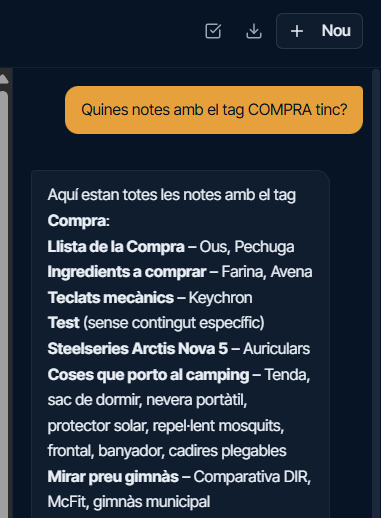
\includegraphics[height=0.7\textheight]{chat-rag.png}
  \end{center}
  \vfill
  \begin{center}
    \small Vídeo complet ($\approx$5:50) a l'annex de la memoria.
  \end{center}
\end{frame}

\begin{frame}{Conclusions}
  \begin{itemize}
    \item \alert{9/9 objectius} assolits; plataforma viva i repositori public.
    \item Si: es pot exposar un magatzem de notes a agents autonoms de forma segura,
      amb \textbf{defensa en capes} i un \textbf{jutge LLM validat empiricament}.
    \item La contribucio central no es una eina, es el \textbf{metode}: analitzar la
      Lethal Trifecta eina per eina i defensar nomes el vector que la satisfa.
  \end{itemize}
\end{frame}

\begin{frame}{Treball futur}
  \begin{itemize}
    \item Jutge \textbf{cross-provider} (Gemini jutja, Anthropic resumeix): mes dificil
      de subvertir amb un sol payload.
    \item Agent \texttt{embedding-backfill} per a corpora 10$\times$ mes grans.
    \item Generalitzar el framework MCP+OAuth a un \textbf{package npm} reutilitzable.
    \item \textbf{Load test} formal multi-tenant (k6 / artillery).
  \end{itemize}
\end{frame}

\begin{frame}[standout]
  Gracies.

  \vspace{0.5cm}
  \small Preguntes?
\end{frame}

\end{document}
